% TEMPLATE for Usenix papers, specifically to meet requirements of
%  USENIX '05
% originally a template for producing IEEE-format articles using LaTeX.
%   written by Matthew Ward, CS Department, Worcester Polytechnic Institute.
% adapted by David Beazley for his excellent SWIG paper in Proceedings,
%   Tcl 96
% turned into a smartass generic template by De Clarke, with thanks to
%   both the above pioneers
% use at your own risk.  Complaints to /dev/null.
% make it two column with no page numbering, default is 10 point

% Munged by Fred Douglis <douglis@research.att.com> 10/97 to separate
% the .sty file from the LaTeX source template, so that people can
% more easily include the .sty file into an existing document.  Also
% changed to more closely follow the style guidelines as represented
% by the Word sample file. 
% This version uses the latex2e styles, not the very ancient 2.09 stuff.
\documentclass[10pt,twocolumn]{report}
\usepackage{graphicx,epsfig,endnotes}
\begin{document}

%don't want date printed
% \date{}

%make title bold and 14 pt font (Latex default is non-bold, 16 pt)
\title{\Large \bf DataSeries User Guide}

% \numberofauthors{0}
%for single author (just remove % characters)
% \author{
% \alignauthor Eric Anderson\\
% \affaddr{HP Labs}\\
% \affaddr{Palo Alto, CA}\\
% \email{eric.anderson4@hp.com}
% \alignauthor Martin Arlitt\\
% \affaddr{HP Labs}\\
% \affaddr{Palo Alto, CA}\\
% \email{martin.arlitt@hp.com}
% \alignauthor Charles B. Morrey III\\
% \affaddr{HP Labs}\\
% \affaddr{Palo Alto, CA}\\
% \email{brad.morrey@hp.com}
% \and
% \alignauthor Alistair Veitch\\
% \affaddr{HP Labs}\\
% \affaddr{Palo Alto, CA}\\
% \email{alistair.veitch@hp.com}
%\and
%{\rm Second Name}\\
%Second Institution
% copy the following lines to add more authors
% \and
% {\rm Name}\\
%Name Institution
% } % end author

\maketitle

% Use the following at camera-ready time to suppress page numbers.
% Comment it out when you first submit the paper for review.
%\thispagestyle{empty}

\section{Introduction}

\fix{11. Another word rather than intense in title?}
\fix{13. More motivation on why we do tracing -- if we can get the space}
Storage tracing and analysis has a long history.  Some of the earliest
filesystem traces were captured in 1985~\cite{ousterhout85}, and there
has been intermittent tracing effort since then, summarized by
Leung~\cite{LeungUsenix08}.  These traces are
analyzed to find properties that future systems should support or
exploit, and as input to simulators and replay tools to explore system
performance with real workloads.

One of the problems
with trace analysis is that old traces inherently have to be scaled up
to be used for evaluating newer storage systems because the
underlying performance of the newer systems has increased.  Therefore,
the community benefits from regularly capturing new traces from multiple
sources, and if possible, traces that put a heavy load on the storage
system, reducing the need to scale the workload.

Most traces, since they are performed by academics, are captured in
academic settings.  This means that the workloads captured are
somewhat comparable, but it also means that commercial workloads are
under-emphasized.  Microsoft is working to correct this by capturing
commercial enterprise traces from their internal
servers~\cite{snia-iotta-microsoft}.  Our work focuses on commercial
NFS~\cite{rfc1094nfs} workloads, in particular from a feature animation (movie) company.
The name of the company remains blinded as part of the agreement to
publish the traces.  The last publically available NFS traces that we
are aware of were collected in 2003.  Our 2003 and 2007
traces~\cite{animation-bear-traces} provide recent NFS traces for use
by the community.

One difference between our traces and other ones is the data rates
that we measured.  Our 2003 client traces saw about 750 million
operations per day.  In comparison, the 2003 Ellard
traces~\cite{EllardLisa03} saw a peak of about 125 million NFS
operations per day, and the 2007 Leung traces~\cite{LeungUsenix08}
saw a peak of 19 million CIFS operations/day.  Our 2007 traces saw
about 2.4 billion operations/day.  This difference required us to
develop and adopt new techniques to capture, convert, and analyze the
traces.

Since our traces were captured in such a different environment than
prior traces, we limit our comparisons to their workloads, and we
do not attempt to make any claims about trends.  We believe that
unless we, as a community, collect traces from hundreds of different
sites, we will not have sufficient data to make claims stronger than
``this workload is different from other ones in these ways.''  In
fact, we make limited comparison in the trends between our 2003 and
2007 traces for similar reasons.  The underlying workload changed
as the rendering techniques improved to generate higher quality output,
the operating system generating the requests changed, the NFS
protocol version changed, and the configuration of the clients 
changed because of standard technology trends.

The process of understanding a workload involves four main
steps, as shown in Figure~\ref{fig:overall-process}.  Our tools for
these steps are shown in italics for each step, as well as some
traditional tools.  The first step is capturing the workload, usually
as some type of trace.  The second step is conversion, ususally from
some raw format into a format designed for analysis.  The third step
is analysis to reduce the huge amount of converted data to
something manageable.  Alternately, this step is a simulation or replay to
explore some new system architecture.  Finally the fourth step is to
generate graphs or textual reports from the output of the analysis or
simulation.

Our work has five main contributions:

\begin{enumerate}
\item The development of techniques for lossless raw packet capture up to
5Gb/s, and with the hardware improvements since our work, likely to
10Gb/s.  These techniques are applicable to anyone wanting to capture
a network storage service such as NFS, CIFS, or iSCSI.

\item A series of guidelines for the conversion and storage of the
traces.  Many of these guidelines are things that we wish we had known
when we were converting our traces.  We used
DataSeries~\cite{DataSeriesOSR2009} to store the traces, but our
guidelines are general.

\item Improved techniques for analyzing very large traces that allow
us to look at the burstiness in workloads, and an examination of how
the long averaging intervals in prior analysis can obscure workload
properties.

\item The analysis of an intense NFS workload demonstrating that our
techniques are successful.

\item The agreement with the animation company to allow the roughly
100 billion operation anonymized traces to be published, along with
the complete set of tools to perform all the analysis presented in
this paper and to generate the graphs.  Other
researchers can build on our tools for further analysis, and use
the traces in simulation studies.
\end{enumerate}

\begin{figure}
\center 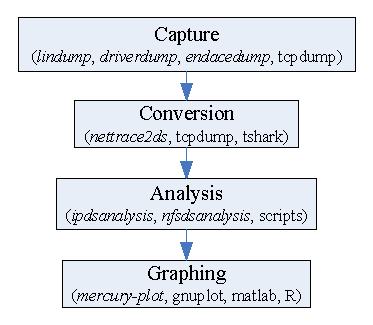
\epsfig{width=2.2in, angle=0, file=overall-process.eps}
\caption{Overall process; our tools are shown in italics, traditional tools
after them.}
\label{fig:overall-process}
\end{figure}

We examine related work in section~\ref{sec:related}.  We describe our
capture techniques in section~\ref{sec:capture}, followed by the
conversion (section~\ref{sec:conversion}). We describe our adopted and
new analysis techniques in section~\ref{sec:analysis-techniques} and
use them to analyze the workload in section~\ref{sec:analysis}.
Finally we conclude in section~\ref{sec:conclusion}.

\chapter{Generic Programs}\label{chap:programs}

There are a number of existing programs present in DataSeries that can
be useful in working with DataSeries files.  We describe when one of
these programs would be used, and sketch the general usage of each
program here.  Detailed usage information on a program can be found on
that programs manual page.

Usually when you download DataSeries files from a remote repository,
the files will have been compressed with bz2\cite{BZIP2} compression.
This is done so that the files will be a small as possible during
transfer. However, bz2 is slow to decompress, and so it is useful to
convert the downloaded files to a faster decompression algorithm, and
sacrifice increased local storage space space.  The {\tt
dsrepack}\ref{program:dsrepack} program will perform this conversion.

The next most common operation is to take a quick look at the
downloaded DataSeries files.  The {\tt ds2txt}\ref{program:ds2txt}
program will take a DataSeries file and convert it to text so that the
type descriptions for the data stored in the file can be seen, and so
that a few of the sample lines can be examined.

A better understading of the data in the file may be gained by looking
at some statistics in the downloaded files.  This can be done by using
the {\tt dsstatgroupby}\ref{program:dsstatgroupby} program to
calculate statistics over various combinations of columns grouped by
another column.  This program can be looked at as a very restrictive
version of the SQL select statement.

Finally, before running a large number of analysis programs over the
downloaded files, it is usually useful to build an index over the
downloaded files.  This step can be performed by running {\tt
dsextentindex}\ref{program:dsextentindex}.  This generates an index
which can efficiently return the extents\ref{file-format:extent}
(sub-file chunks) that contain some amount of the desired data for the
analysis.

\section{{\tt dsrepack} -- re-compressing and merging DataSeries files}
\label{program:dsrepack}

\section{{\tt ds2txt} -- converting DataSeries files to text}
\label{program:ds2txt}

\section{{\tt dsstatgroupby} -- calculating statistics over input data}
\label{program:dsstatgroupby}

\section{{\tt dsextentindex} -- indexing DataSeries files}
\label{program:dsextentindex}



\chapter{Writing an analysis modules}\label{chap:analysis-module}

The most common operation in DataSeries is that you want to perform an analy

\chapter{Existing modules}\label{chap:existing-modules}

\chapter{Writing a conversion program}\label{chap:conversion-programs}

\chapter{Specific analysis programs}\label{chap:specific-analysis}


\section{File format specification}

This section provides a precise specification of the DataSeries
version 1 file format.  A conformant dataseries file must consist of
the following sections, as shown in figure~\ref{fig:dsorg}:

\begin{enumerate}
\item {\bf header}: The header includes the version number and check values.
\item {\bf extent-type extent}: The extent defining the types used in the file.
\item {\bf data extent}: Zero or more extents comprising data types defined in the extent-type extent.
\item {\bf index extent}: An extent indexing the types and locations of each exxtent.
\item {\bf trailer}: The trailer contains the offset of the index extent, and some additonal check values.
\end{enumerate}

A conformant implementation may parse files that are missing the index
or the trailer.  The extent-type extent and index extent are simply
data extents with pre-known types, and so will be described after we
specify the extent format.  A valid file must use the same byte
ordering for all values in a file.  A conformant implementation must
support both big endian and little endian orderings.

\subsection{types}

This specification defines the following types:

\begin{enumerate}
\item {\bf byte}: A one byte (8 bit), value ranging from 0..255
\item {\bf int32}: A four byte (32 bit) signed two's complement value stored in host-byte order.
\item {\bf int64}: An eight byte (64 bit) signed two's complement value stored in host-byte order.
\item {\bf double}: An eight byte (64 bit) IEEE 754 floating point value stored in host-byte order.
\end{enumerate}

\subsection{header}

The DataSeries header is used to validate that a file is being
properly parsed. A conformant implementation should validate the
contents of the header, e.g. by calling isnan on the NaN check value.
The header must consist of the following values:

\begin{enumerate}
\item {\bf file-type}: Four bytes, 'DSv1' in ASCII, 0x44, 0x53, 0x76, 0x31 in hexadecimal
\item {\bf int32 check value}: In file byte order, 0x12345678
  (big endian = 0x12, 0x34, 0x56, 0x78; little endian = 0x78, 0x56, 0x34, 0x12).
\item {\bf int64 check value}: In file byte order, 0x123456789ABCDEF0
  (big endian 0x12 0x34 0x56 0x78 0x9a 0xbc 0xde 0xf0; little endian =
  0xf0 0xde 0xbc 0x9a 0x78 0x56 0x34 0x12).
\item {\bf double check value}: The double constant
  3.1415926535897932384 in file byte order.  (big endian 40 09 21 fb
  54 44 2d 18; little endian 18 2d 44 54 fb 21 09 40)
\item {\bf infinity check value}: The double IEEE +$\infty$ floating
  point constant  (big endian 7f f0 00 00 00 00 00 00; little endian
  00 00 00 00 00 00 f0 7f).
\item {\bf NaN check value}: Any double IEEE NaN floating point
  constant in file byte order.
\end{enumerate}

\subsection{trailer}

The DataSeries trailer is used to locate the index extent.  A
conformant implementation should validate the trailer, but may choose
to tolerate an invalid trailer.  The trailer consists of the following
bytes:

\begin{enumerate}
  \item {\bf constant bytes}: Four bytes, 0xFF, 0xFF, 0xFF, 0xFF.
  \item {\bf index extent size}: int32 in file byte order, byte size of
    the index extent in the file.
  \item {\bf inverse extent size}: int32 in file byte order, bitwise
    complement of the index extent size.
  \item {\bf semi-random bytes}: int32 in file byte order, an arbitrary
    32 bit integer.  The implementation should chose this value derived
    from the extents in a file so that file contents are reproducable.
  \item {\bf index extent offset}: int64 in file byte order, offset in
    bytes from the beginning of the file for the index extent.
  \item {\bf hash bytes}: int32 in file byte order, bob-jenkins lookup-2
    hash~\cite{bob-jenkins-hash-lookup-2} of the above bytes. 
\end{enumerate}

\subsection{extent}

An extent in a dataseries file stores the actual data of a dataseries
file, or the two special extents in the file.  An extent consists of
the following bytes:

\begin{enumerate}

  \item {\bf compressed fixed-data size}: int32 in file byte order,
    byte size of the compressed representation of the fixed data.

  \item {\bf compressed variable-data size}: int32 in file byte order,
    byte size of the compressed representation of the variable data.

  \item {\bf number of records}: int32 in file byte order, count of
    the number of records (rows) in this extent.

  \item {\bf uncompressed variable-data size}: int32 in file byte order, 
    byte size of the variable representation after it has been uncompressed.
   TODO-eric: does this include the 4 0 bytes in the in-memory rep?

  \item {\bf compressed adler32 digest}: int32 in file byte order, 
    adler32 digest of the compressed data.
    TODO-eric: how calculated...

  \item {\bf partly-unpacked bob-jenkins hash}: int32 in file byte order,
    bob-jenkins hash of the data after it has been partly unpacked.
    TODO-eric: how calculated...

  \item {\bf fixed-records compression algorithm}: byte; index of the
    compression algorithm used for the fixed-data.  Valid compression algorithms
    are shown in section~\ref{sec:ff:compression-types}.

  \item {\bf variable-records compression algorithm}: byte; index of the
    compression algorithm used for the variable-data.  Valid compression algorithms
    are shown in section~\ref{sec:ff:compression-types}.

  \item {\bf extent type name length:} byte; length of the extent-type
    name.

  \item {\bf unused zero byte} byte; 0.  (pad to round up the header to multiple of 4 bytes)

  \item {\bf type name} {\it extent type name length} bytes.  Extent
    type name for the current extent.  Must be either one of the two
    pre-defined types, or one of the types defined in the extent-type
    extent.

  \item {\bf padding} 0--3 bytes; sufficient 0 bytes to pad the
    current offset to 4 byte alignment.  For example, if the type name
    is 7 bytes long, the padding would consist of 1 byte of 0.

  \item {\bf compressed fixed-data} {\it compressed fixed-data size}
    bytes.  The compressed bytes storing the fixed data.

  \item {\bf padding} 0--3 bytes; sufficient 0 bytes to pad the
    current offset to 4 byte alignment.  For example, if the
    compressed fixed-data size is 128, there would be no padding.

  \item {\bf compressed variable-data} {\it compressed variable-data size}
    bytes.  The compressed bytes storing the variable data.

  \item {\bf padding} 0--3 bytes; sufficient 0 bytes to pad the
    current offset to 4 byte alignment.  For example, if the
    compressed variable-data size is 9, the padding would consist of 3
    bytes of 0's.
\end{enumerate}

\subsection{Compression types}
\label{sec:ff:compression-types}

TODO-eric: fill-in




\bibliography{references}
\bibliographystyle{abbrv}
\end{document}

